\section{Результаты и обсуждение}
% \subsection{Красители на основе \emph{пара}-диалкиламинобензальдегидов}
% Синтез хромофоров для ИК области спектра требует построения более длинной полиметиновой цепи по сравнению с синтезированными ранее красителями.
% Чаще других используют остатки тиофена. 
% Так, в работе~\cite{Jang2006} описан синтез красителя~\cmpd{Jang} с использованием N,N-дибутиламинобензальдегида в качестве донора с удлиненной тиофенсодержащей полиметиновой цепью и N-замещенного трицианопирролина~(\ac{tcp}) в качестве акцептора.

% \begin{figure}
%     \centering
%     \begin{overpic}{sections/results/img/Jang_chromophore.eps}
%         \put(70, 13){\cmpd{Jang}}
%     \end{overpic}
%     \caption{Структура оригинального хромофора}
%     \label{fig:Jang_chromophore}
% \end{figure}

% Мы воспроизвели этот синтез, однако в качестве дендроидного заместителя в структуру хромофора был введен новый дендроидный заместитель TAFS, синтезированный авторами~\cite{2019}.

% \begin{figure}
%     \centering
%     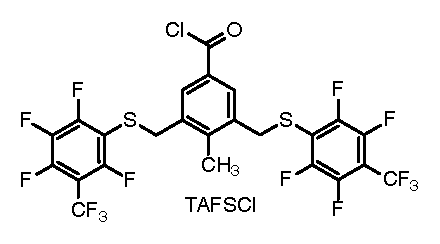
\includegraphics{sections/results/img/TAFS.eps}
%     \caption{Структура TAFS}
%     \label{fig:TAFS}
% \end{figure}

% Схема синтеза хромофора~\cmpd{benzaldehyde_thiophene_TAFS.{dibuthyl}} приведена ниже~(\ref{sch:benzaldehyde_synthesis}). 
% Максимум поглощения красителя в \ce{CHCl3} составляет~\SI{936}{\nano\metre}. 
% Структура соединения подтверждена данными спектров ЯМР~\ce{^1H} и~\ce{^19F}. 
% Характеристическими сигналами в спектре ЯМР~\ce{^1H} соединения~\cmpd{benzaldehyde_thiophene_TAFS.{dibuthyl}} являются два дублета при~\num{8.46} и~\SI{6.83}{\ppm}, образующие \emph{AX}-систему двойной связи, и два дублета при~\num{7.19} и~\SI{7.01}{\ppm}, принадлежащие \emph{AB}-системе второй двойной связи. 
% Константы спин-спинового взаимодействия~(\num{14.8} и~\SI{15.6}{\hertz} соответственно) подтверждают \E-конфигурации обеих связей. 
% Два дублета при~\num{7.43} и~\SI{7.08}{\ppm} с \ac{J}~\SI{4.2}{\hertz} принадлежат протонам тиофена. 
% Кроме того, спектр содержит сигналы протонов двух N-бутильных групп и ароматических протонов пара-фениленового кольца. 
% Спектр ЯМР~\ce{^19F} соответствует структуре TAFS-фрагмента.

% \begin{scheme}
%     \centering
%     \begin{overpic}{sections/results/img/benzaldehyde_synthesis.eps}
%         \put(0, 47){\cmpd{benzaldehyde.{dibuthyl, piperidine}}}
%         \put(25, 43){\cmpd{benzaldehyde_thiophene.{dibuthyl, piperidine}}}
%         \put(50, 39){\cmpd{benzaldehyde_thiophene_CHO.{dibuthyl, piperidine}}}
%         \put(92, 35){\cmpd{benzaldehyde_thiophene_TCP.{dibuthyl, piperidine}}}
%         \put(33, 7){\cmpd{benzaldehyde_thiophene_TAFS.{dibuthyl}}}
%         \put(53, 33){\cmpd{benzaldehyde.{dibuthyl}}\textbf{:}}
%         \put(53, 27){\cmpd{benzaldehyde.{piperidine}}\textbf{:}}
%     \end{overpic}
%     \caption{}
%     \label{sch:benzaldehyde_synthesis}
% \end{scheme}

% При выделении хромофора~\cmpd{benzaldehyde_thiophene_TCP.{dibuthyl}} была получена примесь красно-фиолетового цвета. 
% Мы предполагаем на основании данных спектра ЯМР~\ce{^1H}, что это продукт~\cmpd{benzaldehyde_thiophene_dimer.dibuthyl} конденсации альдегида~\cmpd{benzaldehyde_thiophene_CHO.dibuthyl} с димером малононитрила. Ранее подобные продукты были выделены при конденсации других альдегидов с~\ac{tcp}~\cite{2019}.

% \begin{figure}
%     \centering
%     \begin{overpic}{sections/results/img/byproduct_dimer.eps}
%         \put(52, 0){\cmpd{benzaldehyde_thiophene_dimer.dibuthyl}}
%     \end{overpic}
%     \caption{Стркутура продукта конденсации с димером малононитрила}
% \end{figure}

% Аналогичным способом был синтезирован новый пиперидинозамещенный краситель \cmpd{benzaldehyde_thiophene_TCP.piperidine}. 
% Целевой продукт был получен с меньшим выходом, поскольку образуется гораздо больше побочного продукта на стадии конденсации с~\ac{tcp}.

\subsection{Красители на основе полифтортриарилпиразолинов}
Ранее было показано~\cite{2019, Shelkovnikov2019}, что формильные производные триарилпиразолинов, содержащих полифторфенильные остатки в положениях 5 или 3 пиразолинового цикла, могут служить эффективными донорами в синтезе сопряженных донорно-акцепторных хромофоров с поглощением при 720--760~нм. 
В развитие этой тематики была поставлена задача синтеза Д-А хромофоров c использованием декафторзамещенных производных триарилпиразолина. Наличие двух пентафторфенильных групп дает дополнительные возможности для модификации донорного фрагмента.

Альдегид~\cmpd{decafluoropyrazoline_CHO} был наработан по литературной методике~\cite{2016a,2010}. 
Его получение представляет собой многостадийный процесс~(\ref{sch:decafluoropyrazoline_synthesis}). 
Альдольно-кротоновой конденсацией пентафторацетофенона~\cmpd{perfluorobenzacetophenone} с пентафторбензальдегидом~\cmpd{perfluorobenzaldehyde} получали декафторхалкон~\cmpd{decafluorochalcone}, который переводили в пиразолин~\cmpd{decafluoropyrazoline} конденсацией с фенилгидразином. 
Далее кольцо в положении 1 пиразолина~\cmpd{decafluoropyrazoline} формилировали реакцией Вильсмайера, получая альдегид~\cmpd{decafluoropyrazoline_CHO}.
\begin{scheme}
    \centering
    \begin{overpic}{sections/results/img/decafluoropyrazoline_synthesis.eps}
        \put(7, 40){\cmpd{perfluorobenzacetophenone}}
        \put(30, 40){\cmpd{perfluorobenzaldehyde}}
        \put(71, 40){\cmpd{decafluorochalcone}}
        \put(82, 7){\cmpd{decafluoropyrazoline}}
        \put(22, 8){\cmpd{decafluoropyrazoline_CHO}}
    \end{overpic}
    \caption{Синтез декафторпиразолина}
    \label{sch:decafluoropyrazoline_synthesis}
\end{scheme}

Далее атом фтора в \emph{пара}-положении обоих колец замещали на бифункциональный нулеофил: 4-гидроксипиперидин или пиперазин~(\ref{sch:decafluoropyrazoline_substitution}). 
При~\SI{60}{\celsius} реакция замещения фтора в обеих пентафторфенильных группах на остатки 4-гидроксипиперидина не идет до конца, в смеси присутствует примесь исходного соединения. Поэтому реакционную смесь выдерживали при~\SI{100}{\celsius}. Из реакционной смеси были выделены два соединения~--- целевой альдегид с двумя гидроксипиперидиновыми остатками и альдегид, содержащий в одном из колец диметиламиногруппу. Установить место вступления диметиламиногруппы представляет ближайшую задачу.
Пиперазин вводили при тех же условиях, однако в реакции образуется преимущественно продукт олигомеризации. 
По видимому, требуется бóльший избыток пиперазина.

Спектры ЯМР продукта~\cmpd{decafluoropyrazoline_substituted.piperidine} явно отражают их структуру. 
В спектре ЯМР~\ce{^1H} наблюдаются сигнал альдегдного протона; сигналы системы~\emph{A{A\chemprime}BB\chemprime} \emph{пара}-фениленового кольца; три дублета дублетов, соответствующие системе~\ce{ABX} пиразолинового кольца; в сильном поле~---мультиплеты, соответствующие протонам пиперидиногруппы, в том числе сложный мультиплет, принадлежащий протону \ce{CH-OH}. 
Спектр~\ce{^19F} также имеет характерный вид и содержит уширенный синглет, который соответствует атомам фтора в \emph{орто}-положении кольца в 5 положении пиразолина.
Считается, что это уширение связано с взаимодействием этих атомов фтора с ароматическим кольцом в 1 положении пиразолина.
\begin{scheme}
    \centering
    \begin{overpic}{sections/results/img/fluorine_substitution.eps}
        \put(11, 5){\cmpd{decafluoropyrazoline_CHO}}
        \put(80, 5){\cmpd{decafluoropyrazoline_substituted.{piperidine}}}
    \end{overpic}
    \caption{Замещение атомов фтора на остатки 4-гидроксипиперидина}
    \label{sch:decafluoropyrazoline_substitution}
\end{scheme}

После этого гидроксигруппу альдегида~\cmpd{decafluoropyrazoline_substituted.piperidine} ацилировали~(\ref{sch:ac_cond}).
Были испытаны два подхода: бензоилирование большим избытком хлористого бензоила  и бензоилирование с катализом~\ac{dmap} и стехиометрическим количеством  хлористого бензоила.
В результате было обнаружено, что использование~\ac{dmap} позволяет сократить время реакции с 6--8 часов до 2 в случае хлористого бензоила и требует гораздо меньшего избытка хлорангидрида~(1.25~экв. против 3~экв. при проведении реакции без катализатора).

% О полном ацилировании \ce{OH}-групп можно судить по смещению сигнала протонов \ce{CH-OH} в слабое поле.
\begin{scheme}[ht]
    \centering
    \begin{overpic}{sections/results/img/ac_cond.eps}
        \put(27, 34){\cmpd{decafluoropyrazoline_substituted.piperidine}}
        \put(70, 25){\cmpd{decafluoropyrazoline_benzoyl.piperidine}}
        \put(27, 3){\cmpd{decafluoropyrazoline_benzoyl_DCIF.piperidine}}
    \end{overpic}
    \caption{}
    \label{sch:ac_cond}
\end{scheme}

Также мы исследовали альтернативную последовательность реакций: конденсацию альдегида~\cmpd{decafluoropyrazoline_substituted.piperidine} с дицианоизофороном и последующее ацилирование полученного \mbox{\ce{OH}-красителя}~\cmpd{decafluoropyrazoline_DCIF.piperidine}~(\ref{sch:cond_ac}).

При сопоставимых выходах на стадии ацилирования~(около \SI{60}{\percent}) более выгодным является подход с конденсацией и последующим ацилированием, поскольку он позовляет использовать меньшее количество хлорангидрида, получение которого представляется собой значительную сложность. В итоге оптимизированная последовательность реакций и методика ацилирования позволила снизить требуемое количество ацилирующего реагента.

Мы обнаружили, что при длительной выдержке реакционной смеси вместо пиразолина~\cmpd{decafluoropyrazoline_benzoyl_DCIF.piperidine} образуется соответствующий пиразол. %~\cmpd{decafluoropyrazol_benzoyl_DCIF.piperidine}%~(\ref{sch:pyrazole}).
На образование пиразола указывает отсутствие в \ce{^1H} ЯМР спектре сигналов \emph{ABX}-системы пиразолина и отсутствие в спектре \ce{^19F} уширенного синглета.
\begin{scheme}[ht]
    \centering
    \begin{overpic}{sections/results/img/cond_ac.eps}
        \put(2, 23){\cmpd{decafluoropyrazoline_substituted.piperidine}}
        \put(50, 2){\cmpd{decafluoropyrazoline_DCIF.piperidine}}
        \put(95, 23){\cmpd{decafluoropyrazoline_benzoyl_DCIF.piperidine}}
    \end{overpic}
    \caption{}
    \label{sch:cond_ac}
\end{scheme}

% \begin{scheme}[ht]
%     \centering
%     \begin{overpic}[grid, scale=0.8]{sections/results/img/pyrazole.eps}
%         \put(1, 20){\cmpd{decafluoropyrazoline_DCIF.piperidine}}
%         \put(47, 1){\cmpd{decafluoropyrazol_benzoyl_DCIF.piperidine}}
%     \end{overpic}
%     \caption{}
%     \label{sch:pyrazole}
% \end{scheme}

Также мы наблюдали окисление пиразолина в пиразол даже при кратковременной выдержке в темноте в хлорированных растворителях~(\ce{CH2Cl2} и \ce{CDCl3}).
При этом для предшественника соединения~\cmpd{decafluoropyrazoline_piperidine_DCIF.benzoyl}~--- альдегида~\cmpd{decafluoropyrazoline_substituted.piperidine} окисления не наблюдалось даже при длительной выдержке в хлорофоме на свету. 
Это может быть связано с предполагаемым механизмом окисления~(\ref{sch:light_oxidation} на стр.\,\pageref{sch:light_oxidation}); введение в молекулу акцептора упрощает образование цвиттерионной структуры, играющей ключевую роль в процессе окисления. 
Таким образом, наилучшая стратегия при синтезе и очистке прозводных альдегида~\cmpd{decafluoropyrazoline_substituted.piperidine}~--- избегать хлорсодержащих растворителей.\todo{как-то криво}

\begin{figure}
    \centering
    \begin{overpic}{sections/results/img/dendroids.eps}
        
    \end{overpic}
    \caption{Структуры использованных разделительных блоков}
    \label{fig:dendroids}
\end{figure}
